\documentclass[11pt,a4paper]{article}

\usepackage[T1]{fontenc}
\usepackage[utf8]{inputenc}
\usepackage{lmodern}
\usepackage[margin=2.5cm]{geometry}
\usepackage{microtype}
\usepackage{enumitem}
\usepackage{xcolor}
\usepackage{graphicx}
\usepackage{hyperref}

\graphicspath{{Reports/}{./}}
\setlength{\parindent}{0pt}
\setlength{\parskip}{0.6em}
\setlist[itemize]{topsep=0.2em,itemsep=0.25em}

\definecolor{linkblue}{HTML}{1F4E79}
\hypersetup{
    colorlinks=true,
    linkcolor=linkblue,
    urlcolor=linkblue,
    pdftitle={VIP Week 4 Report},
    pdfauthor={Yorgo Azzi}
}

\begin{document}

\begin{center}
    {\Large\bfseries VIP Week 4 Report}\\[0.5em]
    {\large Yorgo Azzi}\\[0.25em]
    October 7, 2026
\end{center}

\section{Overview}

This week, I expanded the MediaPipe hand interface, made its musical effects
more noticeable, and added a live sheet-music display. I also created a full
architecture diagram showing how OpenCV, MediaPipe, the movement mappings, the
Markov models, SATB generation, MIDI playback, and notation are connected.

The objective was to make the system easier to perform with and easier to
understand. Each hand movement now has a clearer musical result, while the
generated music can be heard and read at the same time.

\section{Work Completed}

\subsection{Expanded Hand Controls}

Volume and rhythmic density were removed from the hand interface because
density was too similar to tempo. The current mappings are:

\begin{itemize}
    \item right-hand height controls the register of all four voices;
    \item left-hand height controls melodic activity;
    \item left-hand horizontal speed controls tempo, using a range designed
    for relatively slow movements so that MediaPipe does not lose the hand;
    \item left-hand openness controls articulation from staccato to legato;
    \item left-hand forward and backward movement controls timbral brightness;
    \item right-hand finger patterns and tilt continue to control chord degree
    and chord quality.
\end{itemize}

The realtime engine was updated so these mappings produce stronger musical
contrasts. High melodic activity now produces more pitch changes and larger
intervals, while low activity permits more stable or repeated notes. Register
has a stronger effect on the target range of each SATB voice. Brightness now
sends both MIDI brightness and resonance controls.

The active camera range was also narrowed to make the controls more sensitive.
The complete height range is reached between 25\% and 75\% of the image, and a
smaller change in apparent palm width now covers the brightness range. Visual
meters were added to the camera window for melodic activity, brightness, and
register.

\subsection{Live Sheet Music}

I added a browser-based live score using \texttt{music21} and Verovio. The
notation comes directly from the same symbolic event generated by the Markov
and SATB engine for MIDI playback; it does not attempt to recognize or
transcribe the audio.

The score shows soprano and alto on the treble staff and tenor and bass on the
bass staff. It includes rhythm, ties, articulation, chord labels, and a red
highlight on the current sonority. The current section contains four measures.
When it is completed, it remains on the page and a new section is added below,
so the complete performance can be reviewed by scrolling backward. A
``Follow live'' button returns the view to the newest measures.

Notation rendering runs on a background thread. MIDI playback therefore does
not wait for MusicXML conversion, SVG engraving, or browser updates. Stem
directions were fixed explicitly to improve readability: soprano and tenor
stems point upward, while alto and bass stems point downward. The staff-name
labels were also removed to provide more space for the music.

\subsection{Architecture Diagram}

I created a complete diagram of the realtime system. It separates the design
into four stages: vision, gesture mapping, music generation, and output. It
also shows that every generated event is sent to two independent paths: MIDI
for sound and an asynchronous queue for live notation.

\begin{figure}[htbp]
    \centering
    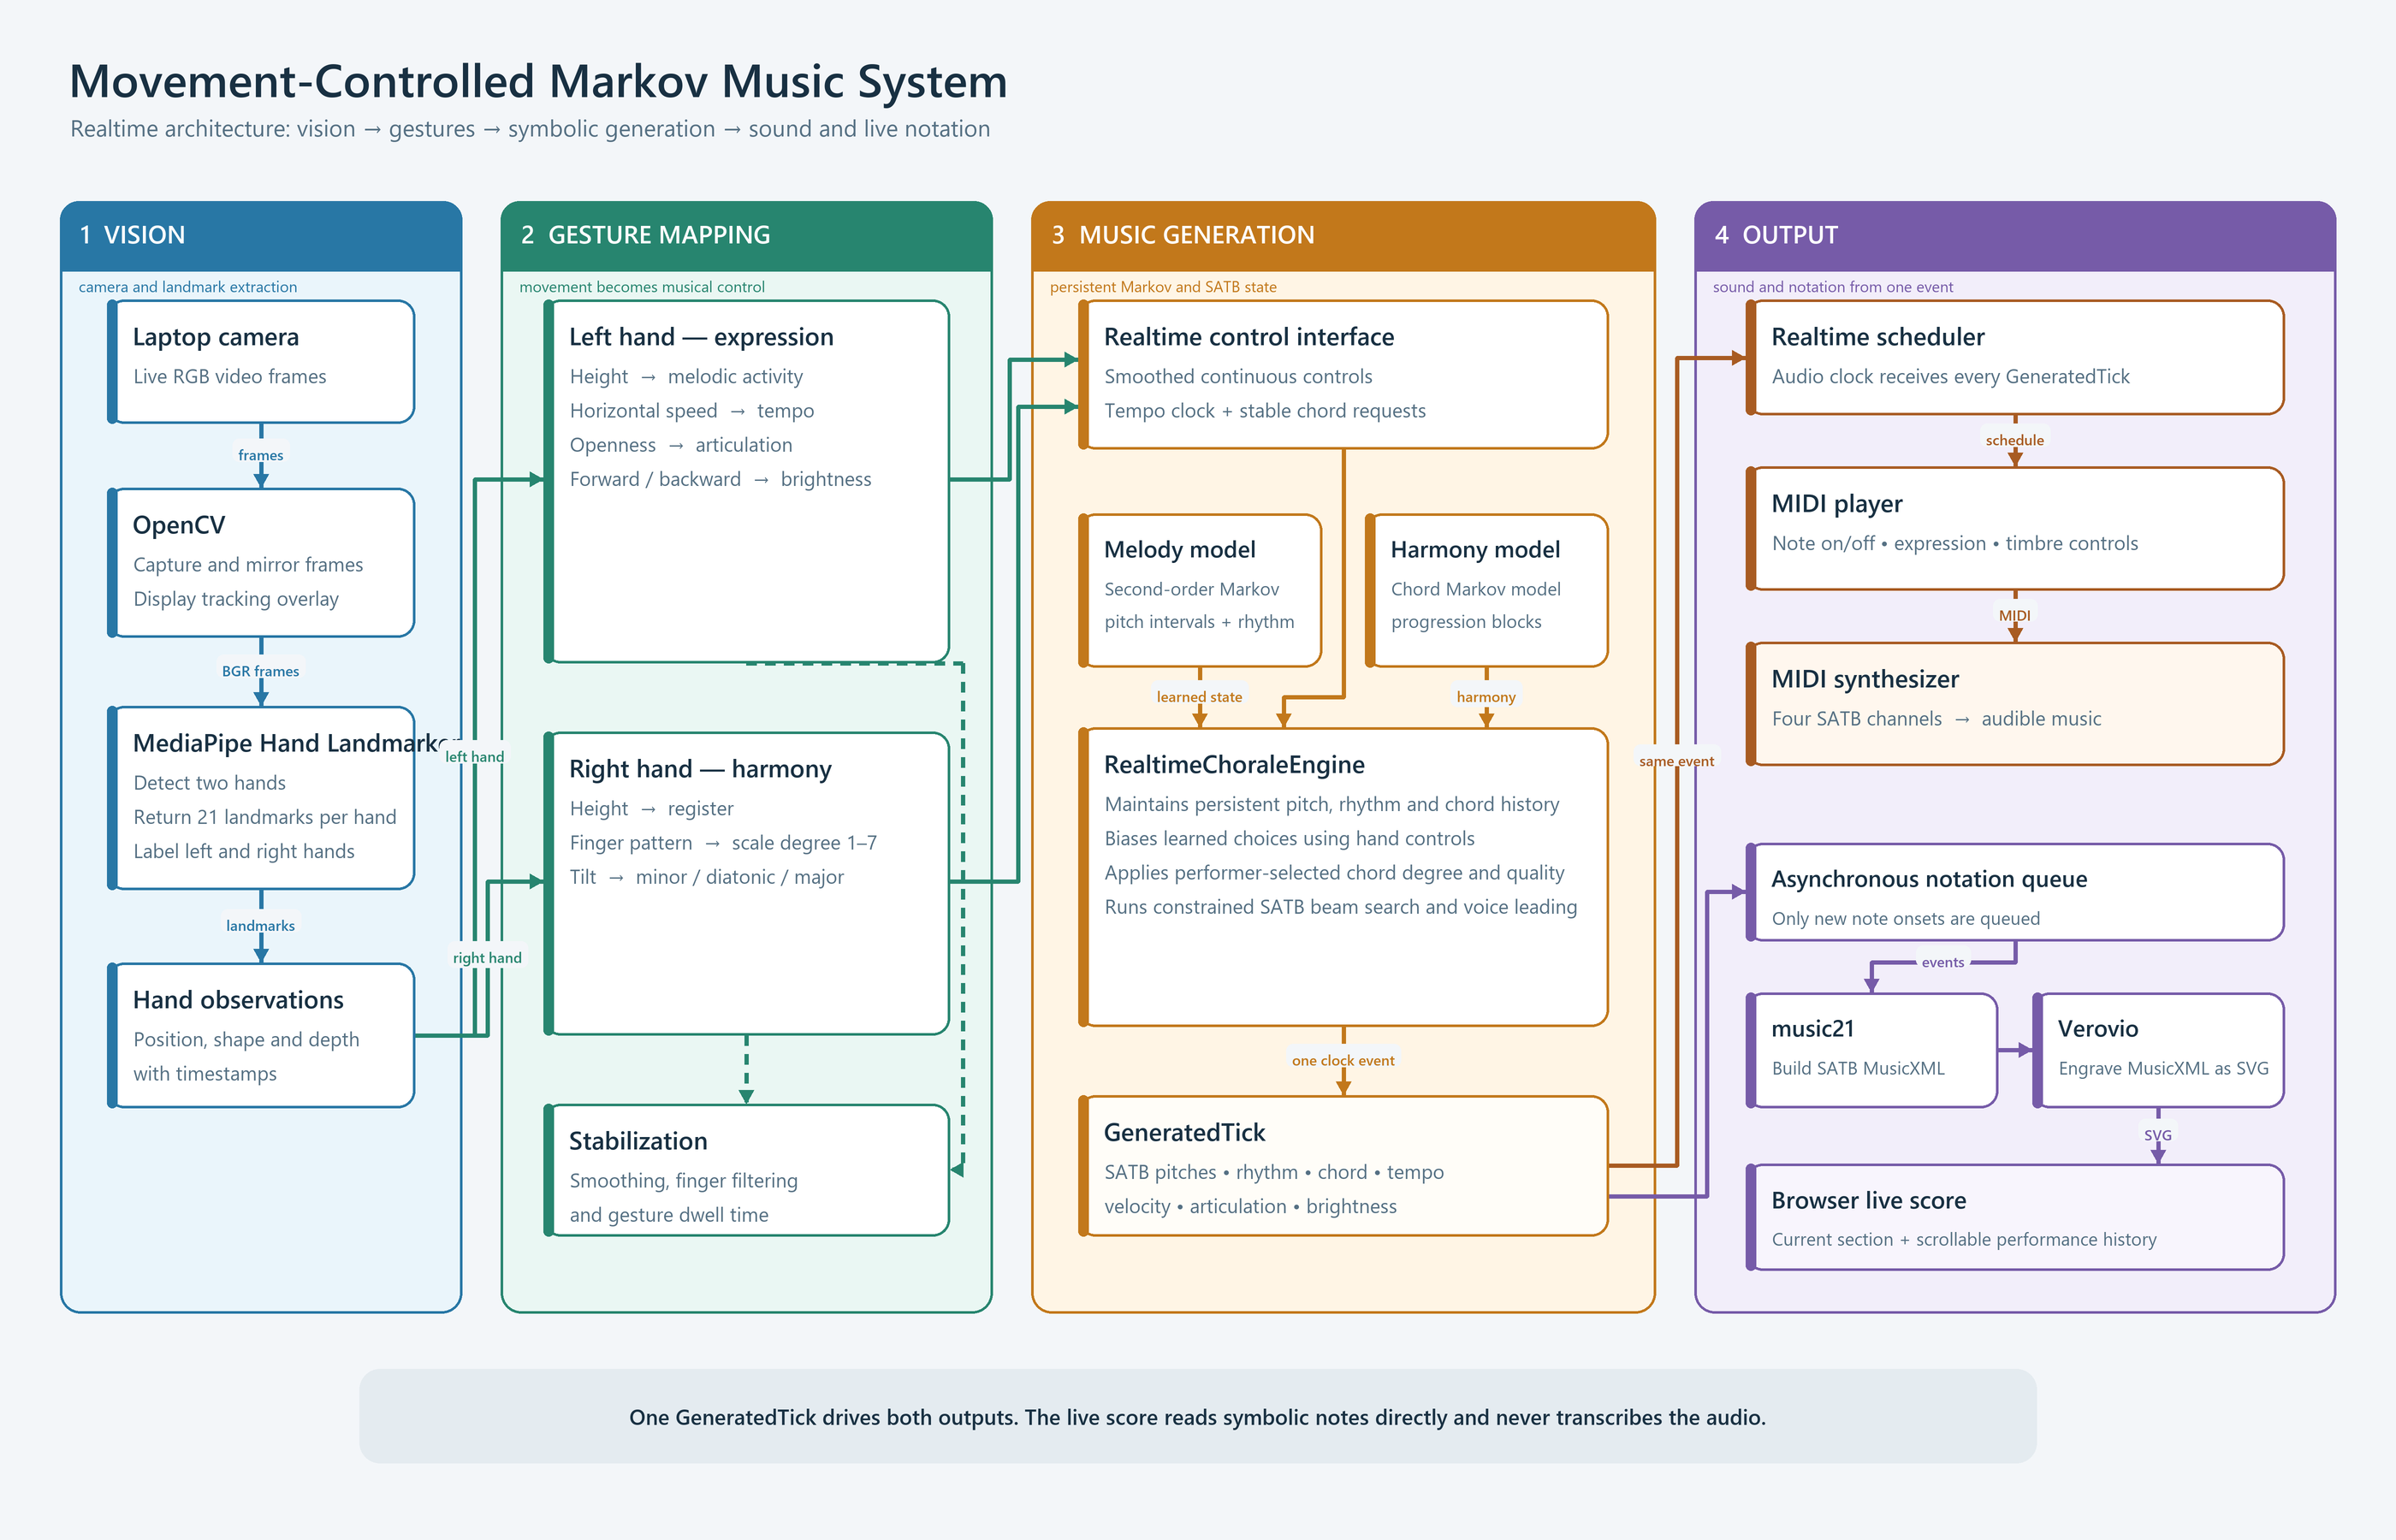
\includegraphics[width=\textwidth]{movement_to_music_architecture.png}
    \caption{Architecture of the movement-controlled Markov music system.}
\end{figure}

\section{Results}

The main results from this week were:

\begin{itemize}
    \item The five continuous movement mappings and the right-hand chord
    gestures operate simultaneously without blocking music generation.
    \item Register tests produced a clear average pitch difference between the
    lowest and highest hand positions.
    \item High melodic activity produced more voice changes than low melodic
    activity under the same generation conditions.
    \item The score remains synchronized because notation and MIDI receive the
    same generated SATB pitches and durations.
    \item Older score sections remain available, allowing the complete
    performance to be reviewed after playing.
    \item Explicit stem directions reduced collisions between the two voices
    sharing each staff.
    \item All 32 automated tests passed, including hand mapping, Markov rhythm,
    chord control, SATB ordering, MIDI expression, live MusicXML generation,
    Verovio rendering, and score-history tests.
\end{itemize}

\section{Challenges}

The main remaining problem is that the musical reaction to the performer's
movement does not always feel immediate. Camera tracking and hand-control
updates run continuously, but the generation engine reads the newest values on
its next clock tick. Controls that affect pitch, register, or melodic activity
usually become audible only when the engine generates the next note onset. A
chord change may wait until the next beat boundary. If the current note has a
long duration, the performer can therefore move a hand without hearing an
instant musical response.

This delay is technically short in many cases, but it weakens the perceived
connection between gesture and sound. The interaction can feel as if the user
is requesting a later change instead of directly shaping the music. Improving
this response is necessary to make the system more satisfying and to give the
performer a stronger sense of musical control.

\section{Next Steps}

\begin{itemize}
    \item Develop a new interaction mode in which the model generates three
    accompaniment voices---alto, tenor, and bass---while the user adds melodic
    fills in the soprano through hand movements. Direct chord control would be
    removed from this mode so the performer can focus on shaping the melodic
    line.
    \item Investigate ways to make gesture responses faster while preserving a
    natural musical flow. Possible directions include shortening or replacing
    a held note when a strong gesture occurs, triggering selected changes
    between regular clock ticks, and designing transitions that respond
    immediately without producing abrupt or disconnected music.
    \item Add a user-interface mode selector. The current full SATB and chord
    control system would remain available, while the new three-voice plus
    performer-controlled soprano mode could be selected from the same
    application.
\end{itemize}

\section{Resources}

\begin{itemize}
    \item Project repository:
    \url{https://github.com/YorgoAzzi/MarkovModel}
    \item MediaPipe Hand Landmarker documentation:
    \url{https://ai.google.dev/edge/mediapipe/solutions/vision/hand_landmarker}
    \item Verovio documentation:
    \url{https://book.verovio.org/}
\end{itemize}

\end{document}
